\documentclass[conference]{IEEEtran}
\IEEEoverridecommandlockouts
\usepackage{cite}
\usepackage{amsmath,amssymb}
\usepackage{graphicx}
\usepackage{booktabs}
\usepackage{xcolor}
\usepackage{algorithm}
\usepackage{algpseudocode}
\usepackage{tikz}
\usetikzlibrary{arrows.meta,positioning}
\usepackage{url}
\usepackage[hidelinks]{hyperref}
\graphicspath{{figures/}}
% Red text marks sentences that must be completed with the numbers from YOUR GPU run.
\newcommand{\fillin}[1]{\textcolor{red}{[#1]}}
\newcommand{\tablefile}[1]{\IfFileExists{tables/#1.tex}{\input{tables/#1.tex}}{\fillin{Table \texttt{\detokenize{#1}} is generated by scripts/07\_make\_report\_assets.py after the GPU run.}}}
\newcommand{\figfile}[3]{\begin{figure}[t]\centering\IfFileExists{figures/#1}{\includegraphics[width=#3]{#1}}{\fbox{\parbox{0.9\columnwidth}{\centering\fillin{\texttt{\detokenize{#1}} is generated after the GPU run}}}}\caption{#2}\label{fig:#1}\end{figure}}

\begin{document}

\title{TrialScreen: Evidence-Grounded Criterion-Level Clinical Trial Eligibility Screening with a Fine-Tuned Small Open Decoder, Explicit KV Caching, Tiled Attention and Speculative Decoding}

\author{\IEEEauthorblockN{\fillin{Your Name}}
\IEEEauthorblockA{\fillin{Roll No.}, Department of Computer Science\\
\fillin{University}, \fillin{email}}}

\maketitle

\begin{abstract}
Screening a patient against every inclusion and exclusion criterion of a clinical trial is slow manual work. We build TrialScreen, an educational prototype that, for each criterion, predicts one of the expert label categories of the TrialGPT Criterion Annotations dataset (including \emph{not enough information} and \emph{not applicable}) and cites the patient sentences that support the decision. We fine-tune the open-weight Qwen2.5-1.5B-Instruct decoder with low-rank adaptation (LoRA) on a fixed 37-patient training split and evaluate on 8 held-out patients. Around the model we implement, from first principles and with tests, (i) a hand-written Qwen2 forward pass with its own key/value (KV) cache, (ii) tiled scaled dot-product attention with an online softmax, and (iii) greedy speculative decoding with a Qwen2.5-0.5B draft and explicit cache rollback. All decoding paths reproduce greedy target tokens exactly in our tests, and our decoder matches the reference library logits to within $2.2\times10^{-4}$ on the real 0.5B model. On the held-out test patients the fine-tuned model reaches \fillin{accuracy X} and \fillin{macro-F1 Y} versus \fillin{X0 / Y0} before fine-tuning. A browser application exposes screening, evidence inspection, report export and a live decoding benchmark.
\end{abstract}

\begin{IEEEkeywords}
clinical trial matching, eligibility, LoRA, KV cache, online softmax, speculative decoding, small language models
\end{IEEEkeywords}

\section{Introduction}
Patient recruitment is a major bottleneck for clinical trials, and eligibility screening is largely manual: each criterion is checked against free-text notes. Large language models (LLMs) can read both the notes and the criteria. TrialGPT~\cite{jin2024trialgpt} showed that GPT-4 can predict criterion-level eligibility with explanations close to expert quality, and Wornow et al.~\cite{wornow2024zeroshot} reported strong zero-shot results on the n2c2 cohort-selection benchmark. Those systems rely on proprietary models; clinical data, cost and reproducibility argue for small models that run locally~\cite{nievas2024distilling}.

\textbf{Problem statement.} Given (i) a patient note split into numbered sentences, (ii) a criterion type (inclusion or exclusion) and (iii) the criterion text, predict the expert eligibility category and the set of supporting sentence IDs, using only freely available hardware and an open-weight model. Missing information must not be treated as proof either way. Because the dataset labels criteria and not whole trials, any trial-level outcome we show is an explicit rule-based aggregation.

\textbf{Contributions.} (1) A leakage-checked, reproducible pipeline on the prescribed patient split with LoRA fine-tuning of Qwen2.5-1.5B-Instruct and a before/after comparison under identical decoding. (2) A hand-written Qwen2 decoder with an explicit pre-allocated KV cache, validated against the library and an uncached reference. (3) Tiled online-softmax attention validated against a float64 reference. (4) Greedy speculative decoding with explicit cache rollback, validated for exact token equality under full, partial and zero draft acceptance. (5) A browser application with evidence highlighting, report export and live inference comparisons.

\section{Related Work}
\textbf{Trial matching with LLMs.} TrialGPT~\cite{jin2024trialgpt} decomposes matching into retrieval, criterion-level matching and trial ranking; its matching module reached 87.3\% accuracy on the 1{,}015 patient--criterion pairs released as the dataset we use. Wornow et al.~\cite{wornow2024zeroshot} studied zero-shot prompting strategies and a retrieval stage that reduces tokens, and had clinicians rate the generated justifications. Nievas et al.~\cite{nievas2024distilling} fine-tuned open LLaMA models on GPT-4-generated synthetic data and reached parity with GPT-3.5. \emph{Limitation relevant to us:} these works use 7B+ or proprietary models and rely on GPT-generated rationales; the assignment forbids GPT-4 outputs as inputs or targets, so we train only on expert labels and evidence sentences and build explanations extractively.

\textbf{Architectures and adaptation.} We use a decoder-only Transformer~\cite{vaswani2017attention} with rotary position embeddings (RoPE)~\cite{su2024roformer} and grouped-query attention (GQA)~\cite{ainslie2023gqa}, as in Qwen2.5~\cite{qwen2025qwen25}. LoRA~\cite{hu2022lora} freezes the base weights and learns a low-rank update; QLoRA~\cite{dettmers2023qlora} adds 4-bit base weights. We chose plain LoRA because a 1.5B model fits a free 16\,GB GPU in full precision, avoiding quantisation error and a dependency (bitsandbytes) that is fragile on some free GPUs.

\textbf{Efficient inference.} KV caching turns each decoding step from $O(t)$ token recomputation into a single-token pass, at the cost of memory that grows linearly with length~\cite{pope2023efficiently}; PagedAttention~\cite{kwon2023paged} manages that memory in blocks for serving. Online softmax~\cite{milakov2018online} computes softmax in one pass with a running maximum and normaliser; Rabe and Staats~\cite{rabe2021selfattention} and FlashAttention~\cite{dao2022flashattention,dao2024flashattention2} use it to avoid materialising the $T\times T$ score matrix. Speculative decoding~\cite{leviathan2023fast,chen2023accelerating} lets a cheap draft model propose tokens that the target verifies in one parallel pass; with greedy acceptance the output is identical to greedy target decoding.

\section{Materials and Methods}
\subsection{Dataset and fixed split}
The TrialGPT Criterion Annotations dataset contains 1{,}015 annotations over 53 synthetic patients (TREC/SIGIR cohorts). Each row has a note whose sentences are numbered from 0, a criterion type and text, the expert eligibility label and the expert evidence sentence IDs. GPT-4 columns (\texttt{gpt4\_explanation}, \texttt{gpt4\_sentences}, \texttt{gpt4\_eligibility}, \texttt{explanation\_correctness}) are dropped immediately after loading, and a test asserts they are absent. Following the protocol, the sorted unique patient IDs are shuffled with \texttt{numpy.random.default\_rng(42)}; the first 37 patients form the training split, the next 8 validation and the last 8 test (Table~\ref{tab:split}). A unit test reproduces the split from the seed, checks there is no patient overlap and that every annotation of a patient is in one split. The manifest (patient IDs, counts, label counts, SHA-256 of the data file) is published in \texttt{data/splits/split\_manifest.json}. One annotation (ID 883, training patient sigir-201519) has an empty criterion text in the released file; it cannot form an input and is excluded from training and recorded in the manifest. Labels are highly imbalanced: \emph{excluded} occurs 10 times in total and never in the test split, so test macro-F1 is averaged over the classes present in the gold labels of each subset (absent classes are reported with support 0).

\tablefile{split}

\subsection{Model selection}
We compared three open decoders that fit a free Kaggle T4 (16\,GB) for LoRA training (Table~\ref{tab:models}). KV memory per token is $2\,L\,H_{kv}\,d_h\,b$ for $L$ layers, $H_{kv}$ KV heads, head size $d_h$ and $b$ bytes per value. Qwen2.5-1.5B-Instruct was selected because (i) its Apache-2.0 licence and ungated download keep the project reproducible, (ii) GQA with 2 KV heads makes its cache about 7$\times$ smaller per token than SmolLM2-1.7B's full multi-head cache, which matters for the KV-cache and speculative experiments, (iii) a smaller sibling (Qwen2.5-0.5B-Instruct) shares the exact 151{,}665-token vocabulary, which we verified programmatically and which speculative decoding requires, and (iv) its 32K context comfortably covers our longest example (610 tokens). Llama-3.2-1B was rejected mainly because it is gated behind a licence acceptance, and its smallest same-tokenizer sibling is not much smaller.

\begin{table}[t]\centering\caption{Candidate open-weight decoders (values from each model's \texttt{config.json}/model card; memory is our estimate).}\label{tab:models}
\resizebox{\columnwidth}{!}{\begin{tabular}{lccc}\toprule
 & Qwen2.5-1.5B-Inst. & SmolLM2-1.7B-Inst. & Llama-3.2-1B-Inst.\\\midrule
Parameters & 1.54B & 1.71B & 1.24B\\
Layers / hidden & 28 / 1536 & 24 / 2048 & 16 / 2048\\
Q / KV heads & 12 / 2 (GQA) & 32 / 32 (MHA) & 32 / 8 (GQA)\\
Context & 32{,}768 & 8{,}192 & 131{,}072\\
Vocabulary & 151{,}936 & 49{,}152 & 128{,}256\\
Licence & Apache-2.0 & Apache-2.0 & Llama 3.2 (gated)\\
fp16 weights & 3.1\,GB & 3.4\,GB & 2.5\,GB\\
KV per token (fp16) & 28\,KB & 192\,KB & 32\,KB\\
Same-vocab draft & Qwen2.5-0.5B & SmolLM2-360M & none smaller\\\bottomrule
\end{tabular}}\end{table}

\subsection{Input/output format and preprocessing}
The input is the Qwen chat template with a short system instruction (use only facts in the note; absence of a fact is not evidence; answer with JSON) and a user message containing the numbered note, the criterion type, the criterion text and the allowed labels for that type. The target is a single JSON object, \texttt{\{"evidence": [ids], "label": "..."\}}. We place evidence before the label so that, autoregressively, the model commits to the cited sentences before the decision. We do not train the model to write free-text rationales: the only rationales in the dataset are GPT-4 outputs, which may not be used. Instead, explanations are built deterministically from the predicted label and the exact cited sentences, so every explanation is traceable to the record. Parsing is strict: IDs outside the note are dropped and logged, a label outside the allowed set is an \emph{invalid output}, and invalid outputs count as errors. With the Qwen tokenizer the longest training example is 610 tokens (mean 315) and the longest target 38 tokens, so with a 1{,}536-token limit \textbf{no example is truncated}; the code raises an error rather than silently truncating, because truncation could remove evidence sentences. Generation uses \texttt{max\_new\_tokens}=48, above the longest target.

\subsection{Fine-tuning}
We apply LoRA~\cite{hu2022lora} to all attention and MLP projections ($W' = W + \frac{\alpha}{r}BA$, $r{=}16$, $\alpha{=}32$, dropout 0.05), training about 18.5M parameters (1.2\% of the model). The loss is next-token cross-entropy on answer tokens only:
\begin{equation}
\mathcal{L} = -\frac{1}{|A|}\sum_{t\in A}\log p_\theta(y_t\mid y_{<t}, x),
\end{equation}
where prompt tokens are masked with label $-100$. We use AdamW (learning rate $2\times10^{-4}$, cosine schedule, 5\% warm-up), effective batch 16 (4$\times$4 accumulation), 3 epochs, gradient clipping 1.0, gradient checkpointing, fp32 master weights with fp16 autocast (the T4 has no bf16), and seed 42. After each epoch we compute validation loss and validation accuracy/macro-F1 by generating answers; the checkpoint with the best validation macro-F1 is kept. The test split is never loaded during training; the evaluation script refuses to touch it without an explicit \texttt{--final} flag.

\subsection{Explicit KV-cached decoding}
Our \texttt{ExplicitQwen2Decoder} re-implements the Qwen2 forward pass (RMSNorm, RoPE, GQA, SwiGLU MLP, tied output head) using the loaded model's weight tensors, so the same code serves the base and LoRA-merged models. It owns a pre-allocated cache $K_\ell, V_\ell \in \mathbb{R}^{1\times H_{kv}\times L_{max}\times d_h}$ per layer and a length pointer $n$.

\emph{Positional handling.} New tokens at absolute positions $n,\dots,n{+}T{-}1$ receive RoPE rotations for those positions \emph{before} their keys are written to the cache, so cached keys never need re-rotation. \emph{Masking.} With $T$ new queries and $n{+}T$ keys, query $i$ may attend to key $j$ iff $j \le n+i$ (a bottom-right aligned causal mask); during single-token decoding this mask is all-true. \emph{Cache growth.} Prefill writes $P$ positions; each decoding step writes one, so memory grows linearly; we report it as $2LH_{kv}d_h b \cdot n$ bytes. Rolling back (needed by speculative decoding) only moves $n$ backwards. GQA is handled by repeating each KV head $H/H_{kv}$ times at attention time, so the cache stores only $H_{kv}$ heads. The reference path without reuse recomputes the whole sequence at every step (Algorithm~\ref{alg:kv}). A second path drives the library's own forward pass with an explicit \texttt{DynamicCache}, passing position IDs ourselves, as an independent cross-check.

\emph{Numerical differences.} Prefill processes many queries in one matrix multiply, while decoding processes one; the different shapes change the order of floating-point reductions, so logits can differ in the last bits, which is amplified in fp16. Greedy outputs differ only if two top logits are within that noise; our benchmark records the step and the top-2 logit margin of any mismatch.

\begin{algorithm}[t]\caption{Greedy decoding with and without cache reuse}\label{alg:kv}
\begin{algorithmic}[1]
\State \textbf{Cached:} $\ell \gets f(x_{1:P})$; cache holds $P$ positions; $y_1\gets\arg\max \ell_P$
\For{$t=2..N$} \State $\ell \gets f(y_{t-1}; \text{cache})$ \Comment{1 token, position $P{+}t{-}2$; cache $+1$}
\State $y_t \gets \arg\max \ell$ \EndFor
\State \textbf{Uncached reference:} for $t=1..N$: $y_t\gets\arg\max f(x_{1:P}, y_{1:t-1})_{\text{last}}$
\end{algorithmic}\end{algorithm}

\subsection{Tiled attention with online softmax}
The reference computes $S = QK^\top/\sqrt{d}$, masks it, subtracts the row maximum and normalises, materialising $T_q\times T_k$ scores. The tiled version streams over key/value tiles of size $B_k$ for each query tile of size $B_q$, keeping per row a running maximum $m$, normaliser $l$ and accumulator $a$:
\begin{align}
m' &= \max(m, \max_j s_j), \quad \alpha = e^{m-m'},\\
l' &= \alpha\, l + \textstyle\sum_j e^{s_j - m'}, \quad a' = \alpha\, a + \textstyle\sum_j e^{s_j-m'}v_j,
\end{align}
and returns $a/l$. Tiles entirely in the causal future are skipped; tiles crossing the diagonal are masked element-wise; fully masked rows are guarded against $-\infty-(-\infty)$. Accumulation is in fp32 (fp64 for fp64 inputs). Memory for scores drops from $O(T_qT_k)$ to $O(B_qB_k)$. The same function can serve as the attention backend of our decoder.

\subsection{Greedy speculative decoding}
Both models keep the invariant that their cache covers all tokens except the newest (Algorithm~\ref{alg:spec}). The draft proposes $k$ tokens; the target scores $[y_{last}, d_1..d_k]$ in one pass, giving its own greedy choices $p_0..p_k$; the longest prefix with $d_i = p_{i-1}$ is accepted and $p_n$ is appended, which is either the target's correction or a free bonus token. Every emitted token is therefore a target argmax, so the output equals greedy target decoding. Rejected positions are removed by cropping both caches. If the per-token acceptance probability is $\alpha$ and a draft step costs $c$ target steps, the expected tokens per round are $(1-\alpha^{k+1})/(1-\alpha)$ and the expected speedup is that quantity divided by $(kc+1)$~\cite{leviathan2023fast}; a speedup therefore needs high agreement and a cheap draft.

\begin{algorithm}[t]\caption{One round of greedy speculative decoding}\label{alg:spec}
\begin{algorithmic}[1]
\Require seq; target cache $=|\text{seq}|-1$
\State draft: feed unprocessed tokens, then generate $d_1..d_k$ greedily
\State $p_{0..k}\gets\arg\max f_{target}([\text{seq}_{-1}, d_1..d_k])$ \Comment{one pass}
\State $n\gets$ largest $n$ with $d_i=p_{i-1}\ \forall i\le n$
\State seq $\gets$ seq $+ [d_1..d_n, p_n]$ \Comment{stop at EOS / budget}
\State crop target cache to $|\text{seq}|-1$; crop draft cache to $\le|\text{seq}|-1$
\end{algorithmic}\end{algorithm}

\subsection{Application workflow}
Fig.~\ref{fig:app} shows the workflow of the browser application (Gradio). A user pastes a note (numbered or free text; free text is split into sentences and numbered), enters criteria under ``Inclusion criteria:'' and ``Exclusion criteria:'' headings, picks a decoding mode and runs the screen. Inputs are validated (empty note, malformed criteria, too many criteria, notes over 2{,}500 tokens are rejected with a message instead of being truncated). Each criterion shows its label, cited sentence IDs and text, and an extractive explanation; the note is displayed with cited sentences highlighted; missing-information criteria and decisions without evidence are listed. A preliminary outcome is produced by an explicit rule: any exclusion predicted \emph{excluded} or inclusion predicted \emph{not included} gives ``likely ineligible''; otherwise any \emph{not enough information} gives ``undetermined''; otherwise ``potentially eligible''. Reports download as HTML and JSON with provenance (model, adapter, decoding settings, timestamp, input hash). A benchmark tab runs all decoding paths live on the same prompt and checks token equality, and an attention tab compares the three attention implementations against fp64.

\begin{figure}[t]\centering
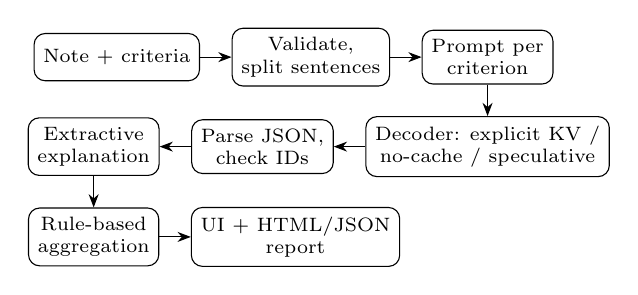
\begin{tikzpicture}[node distance=4mm, every node/.style={font=\scriptsize, draw, rounded corners, align=center, minimum height=6mm}, >=Stealth]
\node (in) {Note + criteria};
\node (val) [right=of in] {Validate,\\split sentences};
\node (pr) [right=of val] {Prompt per\\criterion};
\node (dec) [below=of pr] {Decoder: explicit KV /\\no-cache / speculative};
\node (par) [left=of dec] {Parse JSON,\\check IDs};
\node (exp) [left=of par] {Extractive\\explanation};
\node (agg) [below=of exp] {Rule-based\\aggregation};
\node (out) [right=of agg] {UI + HTML/JSON\\report};
\draw[->] (in)--(val); \draw[->] (val)--(pr); \draw[->] (pr)--(dec); \draw[->] (dec)--(par); \draw[->] (par)--(exp); \draw[->] (exp)--(agg); \draw[->] (agg)--(out);
\end{tikzpicture}
\caption{TrialScreen application workflow.}\label{fig:app}\end{figure}

\section{Experimental Setup and Metrics}
\textbf{Hardware.} Training, evaluation and benchmarks run on one free Kaggle NVIDIA T4 (16\,GB, no bf16), \fillin{PyTorch/transformers versions from results/*.json env field}. Unit tests and a real-model check of the decoder ran on a 1-core CPU. Memory budget: 6.2\,GB fp32 weights for training (plus activations under checkpointing; \fillin{peak from train\_meta.json}\,GB measured); 3.1\,GB fp16 for inference plus 1.0\,GB for the draft.

\textbf{Classification.} Accuracy, macro-F1, per-class precision/recall/F1 and confusion matrices overall and separately for inclusion and exclusion criteria, on the identical examples and decoding settings for the base and fine-tuned models.
\textbf{Evidence.} Predicted and expert ID sets per record. Micro P/R/F1 sums TP, FP and FN over records. Macro P/R/F1 averages over records with a non-empty expert set (an empty prediction there scores 0). Records with an empty expert set (58\% of the data) are reported separately as the share where the model also cites nothing; they are never counted as automatic successes or failures.
\textbf{Efficiency.} Prefill time (to the first token), decode time, tokens per second and peak GPU memory, after one warm-up run, with \texttt{torch.cuda.synchronize()} and the median of 3 runs; EOS is ignored in throughput runs so every path produces the same number of tokens.

\section{Results and Discussion}
\subsection{Fine-tuning}
\figfile{training_curves.png}{Training loss per optimiser step and validation loss / macro-F1 per epoch.}{\columnwidth}
Fig.~\ref{fig:training_curves.png} shows the training curves. \fillin{Describe: how fast the loss falls (the target is short and formulaic, so the JSON format is learned within the first epoch), whether validation loss rises in later epochs (overfitting on 602 examples), and which epoch was selected by validation macro-F1.}

\tablefile{before_after}
Table~\ref{tab:beforeafter} compares the same model before and after fine-tuning under identical prompts and greedy decoding. \fillin{Report the change in valid-JSON rate, accuracy and macro-F1 on validation and test. Typical pattern to check for: the base model often wraps JSON in a code block (handled by our parser), cites every sentence, and over-uses one label; fine-tuning fixes the format and the label vocabulary.}

\subsection{Criterion-level classification and evidence}
\tablefile{perclass_finetuned}
\figfile{confusion_finetuned_test.png}{Test confusion matrices of the fine-tuned model, inclusion (left) and exclusion (right). NEI = not enough information.}{\columnwidth}
\tablefile{evidence_finetuned}
Table~\ref{tab:perclass_finetuned} and Fig.~\ref{fig:confusion_finetuned_test.png} give per-class results on the 8 test patients. \fillin{Discuss: which classes are recognised well (the frequent \emph{not excluded} and \emph{not enough information}) and which fail (rare \emph{not included}, \emph{not applicable}); where confusion concentrates (NEI versus a definite label); and the inclusion versus exclusion difference.} Table~\ref{tab:evidence_finetuned} reports evidence retrieval. \fillin{Discuss precision versus recall of cited sentences and the empty-gold agreement rate.} With only 8 test patients (206 annotations), a single patient's notes can move these numbers by several points, so differences of a few points should not be over-interpreted.

\subsection{Error analysis}
\tablefile{error_categories}
Table~\ref{tab:errcat} groups the test disagreements produced by \texttt{scripts/07\_make\_report\_assets.py}; \texttt{results/error\_cases.md} lists each case. \fillin{Write at least eight distinct cases from error\_cases.md, e.g.: (1) over-confident decision where the note lacks the fact; (2) a decision with no cited evidence (unsupported); (3) a contradictory polarity error (included vs not included); (4) applicability confusion (e.g., a pregnancy criterion for a male patient); (5) right label but wrong evidence sentence; (6) a temporal criterion (``within 6 months'') misread; (7) a numeric threshold criterion; (8) a negated finding in the note (``denies smoking''). For each, quote the criterion, the cited sentence and why the model failed.} We also note a dataset artefact: every note ends with a templated sentence that the patient will consent and comply, which experts cite for consent-type criteria; such criteria are easy and inflate inclusion accuracy.

\subsection{KV-cached decoding}
Before the GPU run we validated the decoder on the real Qwen2.5-0.5B-Instruct (fp32, CPU, a 331-token screening prompt): the maximum absolute logit difference from the library's forward pass was $1.7\times10^{-4}$ with our reference attention, $2.1\times10^{-4}$ with tiled attention and $0$ with PyTorch SDPA, the argmax matched at every position, and greedy generation produced identical tokens with no cache, with our cache and with the library cache. Even on one CPU core, the cached path took 7.2\,s versus 61.7\,s for full recomputation (24 tokens). On tiny random Qwen2 models, unit tests confirm greedy equality for three input/output length pairs and that feeding tokens one by one through the cache reproduces the full-pass logits.
\tablefile{kv_bench}
\figfile{kv_bench.png}{KV-cache benchmark: throughput versus output length and peak memory versus sequence length.}{\columnwidth}
Table~\ref{tab:kv} and Fig.~\ref{fig:kv_bench.png} give the T4 results. \fillin{Discuss: prefill time is similar for all paths (same first pass); uncached decode time grows roughly quadratically with output length because step $t$ processes $P{+}t$ tokens, while cached decode grows linearly; give the speedup at 1024 in / 256 out; memory: the cache adds 28\,KB per token in fp16, small compared with the 3.1\,GB of weights, while the uncached path's activations grow with the recomputed length; report any token mismatch and its top-2 margin.} Our explicit decoder is \fillin{slightly slower / similar} to the library path because it is a Python re-implementation without fused kernels.

\subsection{Tiled attention}
\tablefile{attention_err}
\tablefile{attention_perf}
\figfile{attention_perf.png}{Attention runtime and extra peak memory versus sequence length (log scales).}{\columnwidth}
On CPU, all 28 correctness cases (7 shapes $\times$ causal/non-causal $\times$ fp32/bf16, including single-query decoding, rectangular bottom-right masks and tile sizes that do not divide the length) passed, with a maximum fp32 error against the fp64 reference of $8.9\times10^{-7}$. Tables~\ref{tab:attn_err}--\ref{tab:attn_perf} and Fig.~\ref{fig:attention_perf.png} give the GPU results. \fillin{Discuss: the reference's memory grows quadratically and \fillin{runs out / grows to X MB} at 4096, the tiled version's grows linearly; the tiled version is nevertheless slower than PyTorch SDPA.} The slowdown is expected: our Python loop launches several small kernels per tile and writes intermediate tiles to global memory, whereas fused kernels such as FlashAttention~\cite{dao2022flashattention} keep tiles in on-chip SRAM, fuse the exponentials, rescaling and matrix products into one kernel and parallelise over tiles. The algorithm, not our implementation, is what saves memory traffic.

\subsection{Speculative decoding}
\tablefile{speculative}
\figfile{speculative.png}{Speedup over greedy target decoding and draft acceptance rate versus lookahead $k$.}{0.85\columnwidth}
Unit tests show token equality with greedy target decoding for $k\in\{1,3,5\}$ with an identical draft (acceptance 1.0), a perturbed draft (partial acceptance, exercising rejection and cache rollback), an unrelated draft (acceptance 0) and EOS inside an accepted block, for both decoder implementations. Table~\ref{tab:spec} and Fig.~\ref{fig:speculative.png} give T4 results. \fillin{Discuss: token equality rate; acceptance on the screening task (the untuned 0.5B draft has not learned our JSON format, so acceptance may be low) versus the free-text summary; why speed-up is limited: at batch size 1 a 1.5B model is not compute-bound on a T4, so a 0.5B draft costs a large fraction $c$ of a target step; the outputs are short (about 15 tokens); and Python overhead per round. State the best $k$.} Fine-tuning the draft on the same data (supported by our training script) is the obvious way to raise acceptance.

\subsection{Application}
\fillin{Insert 2--3 screenshots: screening results with highlighted evidence; the benchmark tab; the exported HTML report.} The application runs without any notebook: it starts with one command or as a hosted Hugging Face Space, downloads the adapter from the Hub and recovers from invalid inputs with explanatory messages.

\section{Limitations}
The test set has 8 patients, so metrics have wide uncertainty and the \emph{excluded} class cannot be evaluated at all. Patients are synthetic and notes short (at most 14 sentences), unlike real records; long records would need retrieval of relevant passages and could exceed the context we validated. Labels are imbalanced, so a model can score well by favouring frequent classes; macro-F1 exposes this but the rare classes have very few training examples. The extractive explanations are faithful to cited text but cannot express reasoning (for example, why a lab value meets a threshold). Our explicit decoder and speculative decoder support batch size 1 only. Benchmarks are on one GPU type. The system has not been validated clinically and must not be used for enrolment decisions; automated screening could also encode biases of the annotations.

\section{Conclusion}
We fine-tuned a small open decoder for criterion-level, evidence-citing eligibility screening on the prescribed TrialGPT split and built and validated the inference machinery around it: an explicit KV-cached decoder, tiled online-softmax attention and greedy speculative decoding, all producing tokens identical to their references. \fillin{One sentence with the main test result and the main efficiency result.} Future work: fine-tuning the draft model, retrieval for long records, and calibrated abstention.

\section*{Appendix: Use of AI Assistance}
\fillin{Describe honestly, e.g.: Claude (Anthropic) was used to help design the repository structure, draft code for data preparation, decoding, attention, speculative decoding and the application, write unit tests, and draft this report. I reviewed and ran all code, verified every number against the logs in results/, fixed issues found during my runs, and can explain and modify each component.} All results in this paper come from our own runs; no TrialGPT outputs are used as inputs, targets or results.

\bibliographystyle{IEEEtran}
\bibliography{refs}
\end{document}
